\documentclass{beamer}
\usepackage[utf8]{inputenc}
\usepackage{graphicx, epsfig}
\usepackage{amsmath,mathrsfs,amsfonts,amssymb}
\usepackage{floatflt}
\usepackage{epic,ecltree}
\usepackage{mathtext}
\usepackage{fancybox}
\usepackage{fancyhdr}
\usepackage{multirow}
\usepackage{enumerate}
\usepackage{epstopdf}
\usepackage{multicol}
\usepackage{algorithm}
\usepackage[noend]{algorithmic}
\usepackage{tikz}
\usepackage{blindtext}
\usetheme{default}%{Singapore}%{Warsaw}%{Warsaw}%{Darmstadt}
\usecolortheme{default}

\setbeamerfont{title}{size=\Huge}
\setbeamertemplate{footline}[page number]{}

\setbeamertemplate{section in toc}[sections numbered]


\makeatletter
\newcommand\HUGE{\@setfontsize\Huge{35}{40}}
\makeatother    

\setbeamerfont{title}{size=\HUGE}
\beamertemplatenavigationsymbolsempty

% latin bold lower
\newcommand{\ba}{\mathbf{a}} 
\newcommand{\bc}{\mathbf{c}} 
\newcommand{\be}{\mathbf{e}} 
\newcommand{\bh}{\mathbf{h}} 
\newcommand{\bp}{\mathbf{p}} 
\newcommand{\bt}{\mathbf{t}} 
\newcommand{\bs}{\mathbf{s}} 
\newcommand{\bu}{\mathbf{u}} 
\newcommand{\bv}{\mathbf{v}} 
\newcommand{\bw}{\mathbf{w}} 
\newcommand{\bx}{\mathbf{x}} 
\newcommand{\by}{\mathbf{y}} 
\newcommand{\bz}{\mathbf{z}} 

% latin bold upper
\newcommand{\bA}{\mathbf{A}} 
\newcommand{\bB}{\mathbf{B}} 
\newcommand{\bC}{\mathbf{C}} 
\newcommand{\bI}{\mathbf{I}} 
\newcommand{\bJ}{\mathbf{J}} 
\newcommand{\bL}{\mathbf{L}} 
\newcommand{\bM}{\mathbf{M}} 
\newcommand{\bP}{\mathbf{P}}
\newcommand{\bQ}{\mathbf{Q}} 
\newcommand{\bR}{\mathbf{R}} 
\newcommand{\bT}{\mathbf{T}} 
\newcommand{\bU}{\mathbf{U}} 
\newcommand{\bV}{\mathbf{V}} 
\newcommand{\bW}{\mathbf{W}} 
\newcommand{\bX}{\mathbf{X}} 
\newcommand{\bY}{\mathbf{Y}} 
\newcommand{\bZ}{\mathbf{Z}} 

% latin cal upper
\newcommand{\cF}{\mathcal{F}} 
\newcommand{\cG}{\mathcal{G}} 
\newcommand{\cI}{\mathcal{I}} 
\newcommand{\cL}{\mathcal{L}} 
\newcommand{\cM}{\mathcal{M}} 
\newcommand{\cN}{\mathcal{N}} 
\newcommand{\cS}{\mathcal{S}} 
\newcommand{\cT}{\mathcal{T}} 
\newcommand{\cW}{\mathcal{W}} 
\newcommand{\cX}{\mathcal{X}} 
\newcommand{\cZ}{\mathcal{Z}} 

% latin bb upper
\newcommand{\bbE}{\mathbb{E}} 
\newcommand{\bbI}{\mathbb{I}} 
\newcommand{\bbP}{\mathbb{P}} 
\newcommand{\bbR}{\mathbb{R}} 

% greek bold lower
\newcommand{\bepsilon}{\boldsymbol{\epsilon}} 
\newcommand{\btheta}{\boldsymbol{\theta}} 
\newcommand{\blambda}{\boldsymbol{\lambda}} 
\newcommand{\bpi}{\boldsymbol{\pi}} 
\newcommand{\bmu}{\boldsymbol{\mu}} 
\newcommand{\bsigma}{\boldsymbol{\sigma}} 
\newcommand{\bphi}{\boldsymbol{\phi}} 

% greek bold upper
\newcommand{\bSigma}{\boldsymbol{\Sigma}} 

\DeclareMathOperator*{\argmin}{arg\,min}
\DeclareMathOperator*{\argmax}{arg\,max}

\newcommand{\createdgmtitle}[1]{\title[\hbox to 56mm{Deep Generative Models  \hfill\insertframenumber\,/\,\inserttotalframenumber}]
	{\vspace{1cm} \\ Deep Generative Models \\ {\Huge Lecture #1}}
	\author{Roman Isachenko}
	\institute{
	Moscow Institute of Physics and Technology
	} 
	\date{2023, Autumn}
}

\usepackage{tikz}
\usetikzlibrary{arrows,shapes,positioning,shadows,trees}

\newcommand\myfootnote[1]{%
  \tikz[remember picture,overlay]
  \draw (current page.south west) +(1in + \oddsidemargin,0.5em)
  node[anchor=south west,inner sep=0pt]{\parbox{\textwidth}{%
      \rlap{\rule{10em}{0.4pt}}\raggedright\scriptsize \textit{#1}}};}

\newcommand\myfootnotewithlink[2]{%
  \tikz[remember picture,overlay]
  \draw (current page.south west) +(1in + \oddsidemargin,0.5em)
  node[anchor=south west,inner sep=0pt]{\parbox{\textwidth}{%
      \rlap{\rule{10em}{0.4pt}}\raggedright\scriptsize\href{#1}{\textit{#2}}}};}
      
\AtBeginSection[]
      {
      	\begin{frame}{Outline}
      		\tableofcontents[currentsection]
      	\end{frame}
      }
      \AtBeginSubsection[]{
      	\begin{frame}{Outline}
      		\tableofcontents[currentsection,currentsubsection]
      	\end{frame}
}
\createdgmtitle{14}

\usepackage{tikz}

\usetikzlibrary{arrows,shapes,positioning,shadows,trees}
%--------------------------------------------------------------------------------
\begin{document}
%--------------------------------------------------------------------------------
\begin{frame}[noframenumbering,plain]
%\thispagestyle{empty}
\titlepage
\end{frame}
%=======
\begin{frame}{Recap of previous lecture}
	\begin{figure}
		\centering
		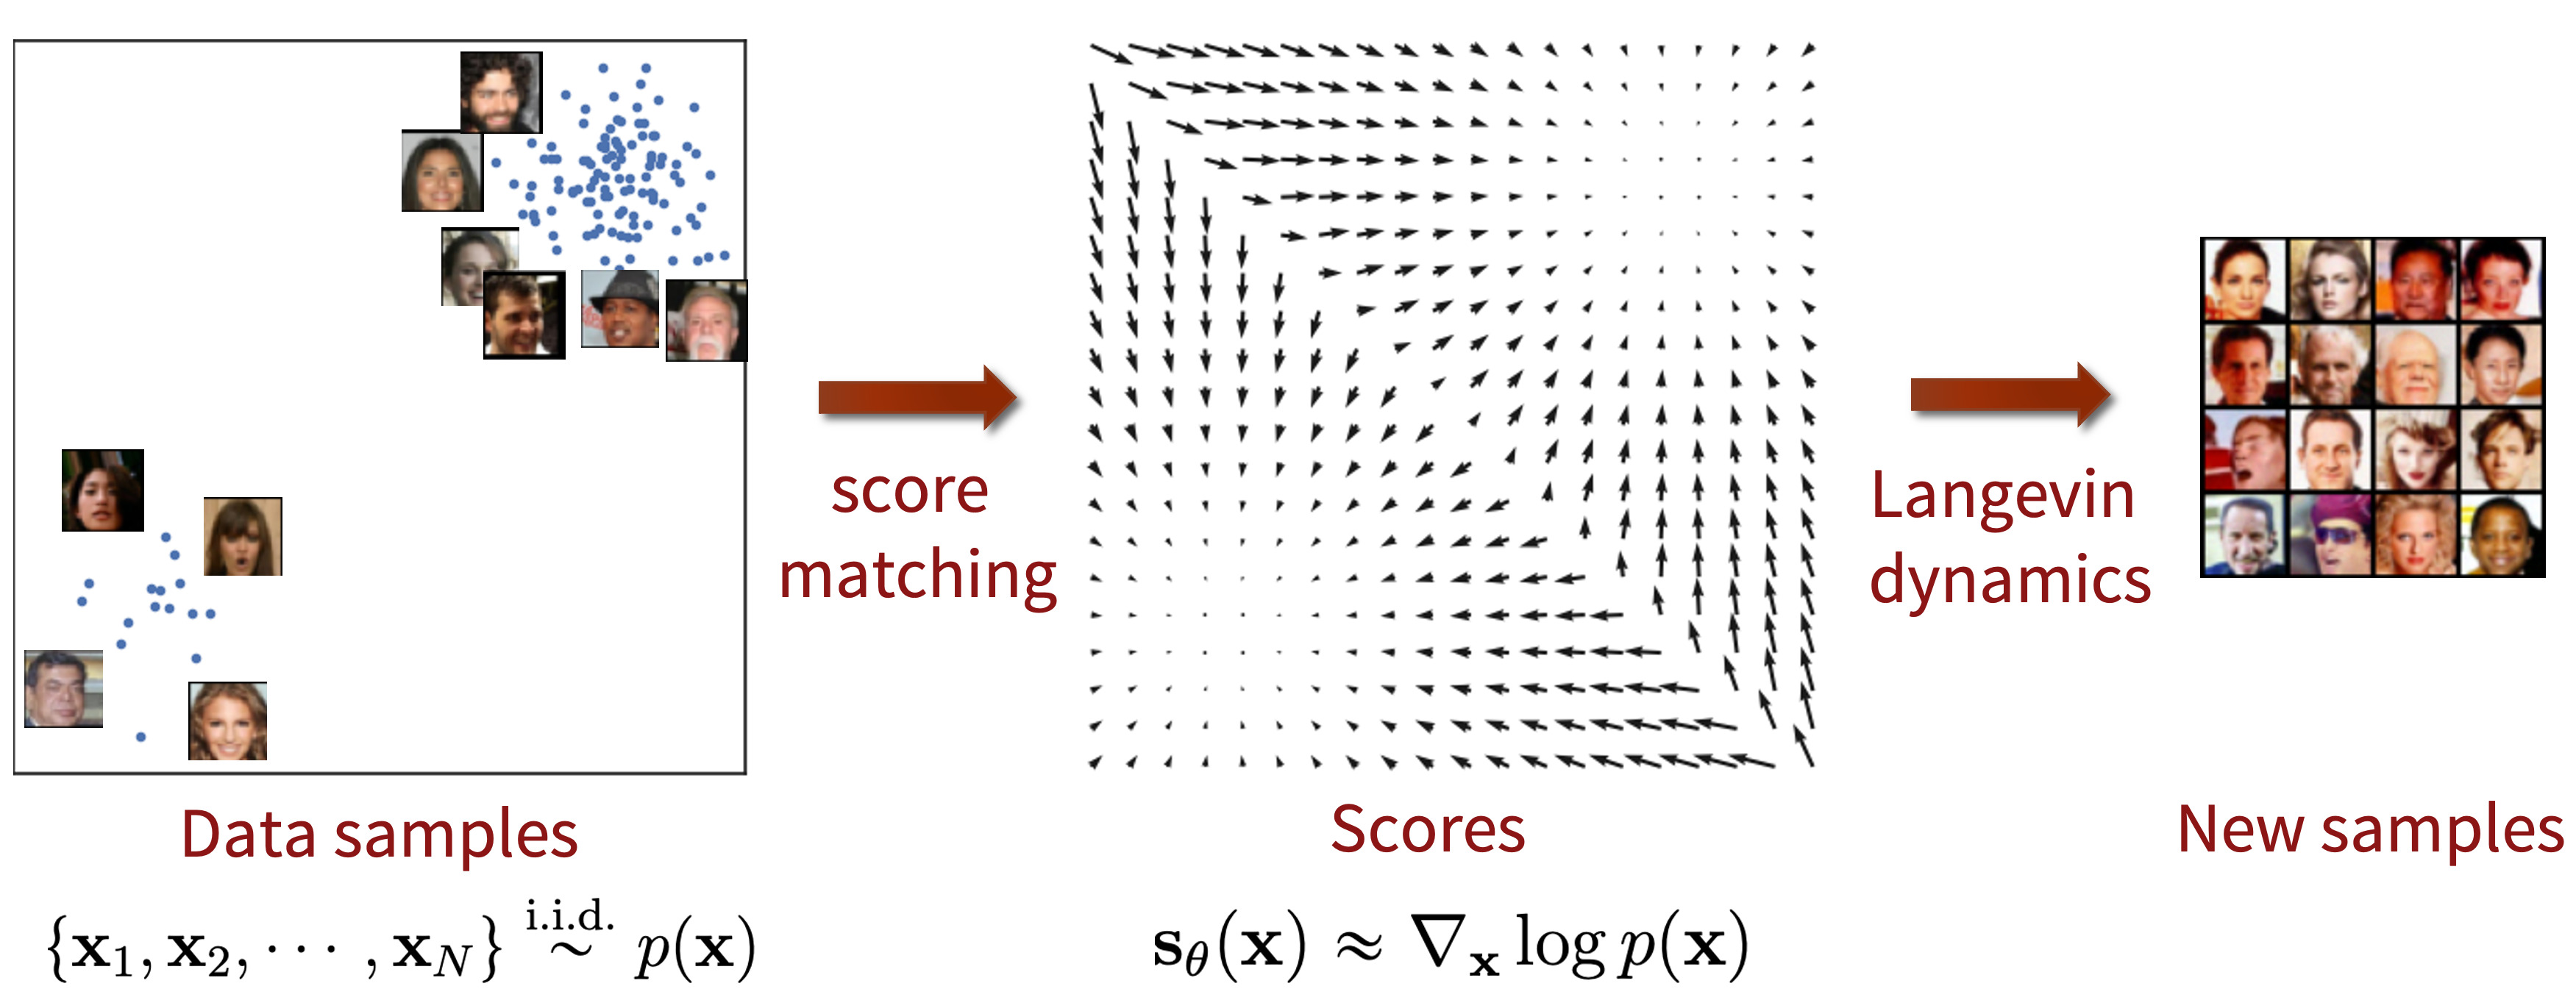
\includegraphics[width=0.75\linewidth]{figs/smld}
	\end{figure}
	\vspace{-0.3cm} 
	\begin{block}{Theorem (implicit score matching)}
		\vspace{-0.6cm}
		\[
		{\color{violet}\frac{1}{2} \bbE_{\pi}\bigl\| \bs(\bx, \btheta) - \nabla_\bx \log \pi(\bx) \bigr\|^2_2} = {\color{teal}\bbE_{\pi}\Bigr[ \frac{1}{2}\| \bs(\bx, \btheta) \|_2^2 + \text{tr}\bigl(\nabla_{\bx} \bs(\bx, \btheta)\bigr) \Bigr]} + \text{const}
		\]
	\end{block}
	\vspace{-0.5cm}
	\begin{enumerate}
		\item {\color{violet}The left hand side} is intractable due to unknown $\pi(\bx)$ -- \textbf{denoising score matching}. 
		\item {\color{teal}The right hand side} is complex due to Hessian matrix -- \textbf{sliced score matching (Hutchinson's trace estimation)}.
	\end{enumerate}
	\myfootnotewithlink{https://yang-song.github.io/blog/2021/score/}{Song Y. Generative Modeling by Estimating Gradients of the Data Distribution, blog post, 2021}
\end{frame}
%=======
\begin{frame}{Recap of previous lecture}
	Let perturb original data by normal noise $p(\bx' | \bx, \sigma) = \cN(\bx' | \bx, \sigma^2 \bI)$
	\vspace{-0.3cm}
	\[
	\pi(\bx' | \sigma) = \int \pi(\bx) p(\bx' | \bx, \sigma) d\bx.
	\]
	\vspace{-0.6cm} \\
	Then the solution of 
	\vspace{-0.2cm}
	\[
	\frac{1}{2} \bbE_{\pi(\bx' | \sigma)}\bigl\| \bs(\bx', \btheta, \sigma) - \nabla_{\bx'} \log \pi(\bx' | \sigma) \bigr\|^2_2 \rightarrow \min_{\btheta}
	\]
	\vspace{-0.5cm} \\
	satisfies $\bs(\bx', \btheta, \sigma) \approx \bs(\bx', \btheta, 0) = \bs(\bx', \btheta)$ if $\sigma$ is small enough.
	\begin{block}{Theorem (denoising score matching)}
		\vspace{-0.8cm}
		\begin{multline*}
			\bbE_{\pi(\bx' | \sigma)}\bigl\| \bs(\bx', \btheta, \sigma) - \nabla_{\bx'} \log \pi(\bx' | \sigma) \bigr\|^2_2 = \\ = \bbE_{\pi(\bx)} \bbE_{p(\bx' | \bx, \sigma)}\bigl\| \bs(\bx', \btheta, \sigma) - \nabla_{\bx'} \log p(\bx' | \bx, \sigma) \bigr\|^2_2 + \text{const}(\btheta)
		\end{multline*}
		\vspace{-0.8cm}
	\end{block}
	Here $\nabla_{\bx'} \log p(\bx' | \bx, \sigma) = - \frac{\bx' - \bx}{\sigma^2}$.
	\begin{itemize}
		\item The RHS does not need to compute $\nabla_{\bx'} \log \pi(\bx' | \sigma)$ and even more $\nabla_{\bx'} \log \pi(\bx')$.
		\item $\bs(\bx', \btheta, \sigma)$ tries to \textbf{denoise} a corrupted sample.
		\item Score function $\bs(\bx', \btheta, \sigma)$ parametrized by $\sigma$. 
	\end{itemize}
	\myfootnotewithlink{http://www.iro.umontreal.ca/~vincentp/Publications/smdae_techreport.pdf}{Vincent P. A Connection Between Score Matching and Denoising Autoencoders, 2010}
\end{frame}
%=======
\begin{frame}{Recap of previous lecture}
	\begin{block}{Noise conditioned score network}
		\begin{itemize}
			\item Define the sequence of noise levels: $\sigma_1 > \sigma_2 > \dots > \sigma_L$.
			\item Train denoised score function $\bs(\bx', \btheta, \sigma)$ for each noise level:
			\vspace{-0.3cm}
			\[
				\sum_{l=1}^L {\color{violet}\sigma_l^2} \bbE_{\pi(\bx)} \bbE_{p(\bx' | \bx, \sigma_l)}\bigl\| \bs(\bx', \btheta, \sigma_l) - \nabla_\bx' \log p(\bx' | \bx, \sigma_l) \bigr\|^2_2 \rightarrow \min_{\btheta}
			\]
			\vspace{-0.5cm}
			\item Sample from \textbf{annealed} Langevin dynamics (for $l=1, \dots, L$).
		\end{itemize}
	\end{block}
	\begin{figure}
		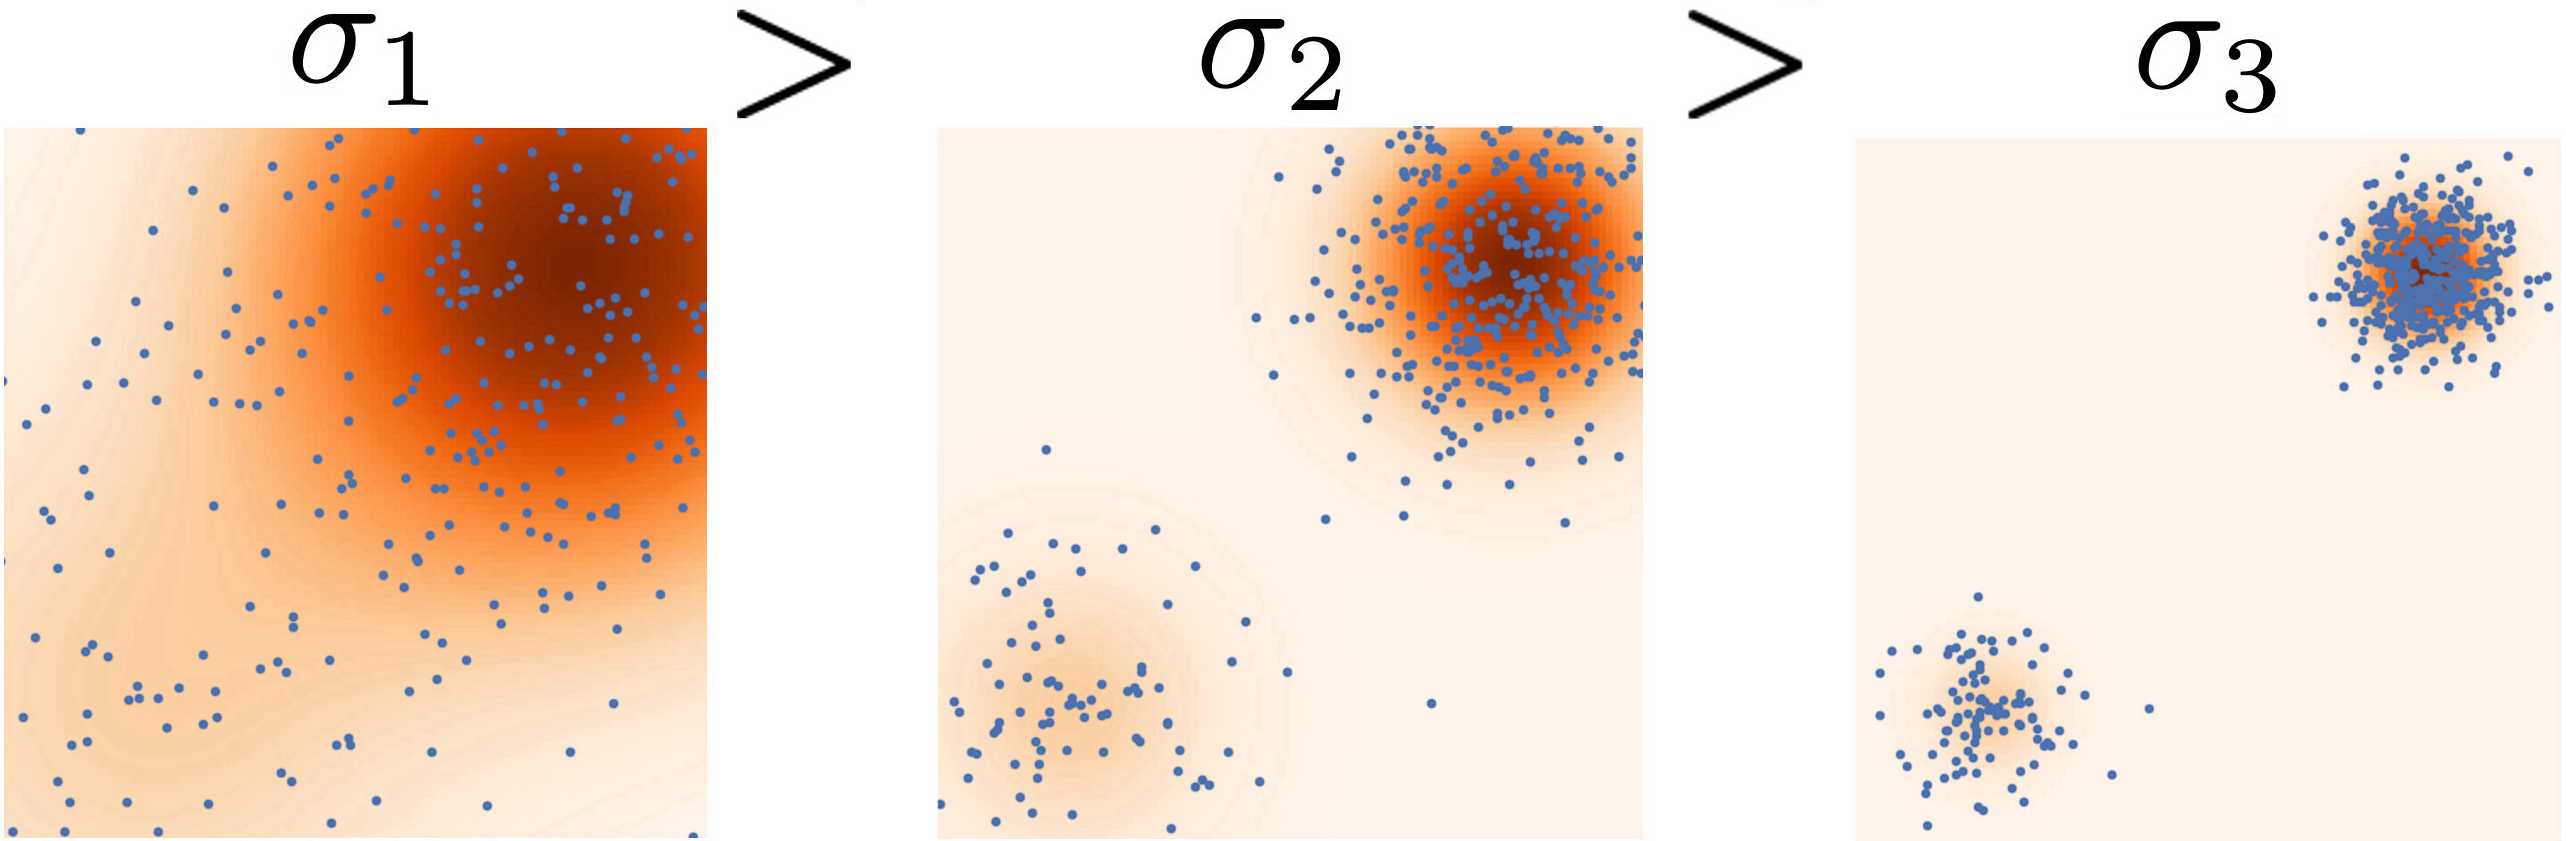
\includegraphics[width=0.55\linewidth]{figs/multi_scale}
	\end{figure}
	\begin{figure}
		
\includegraphics[width=\linewidth]{figs/duoduo}
	\end{figure}
	\myfootnotewithlink{https://arxiv.org/abs/1907.05600}{Song Y. et al. Generative Modeling by Estimating Gradients of the Data Distribution, 2019}
\end{frame}
%=======
\begin{frame}{Recap of previous lecture}
	\begin{block}{Forward gaussian diffusion process}
		\vspace{-0.4cm}
		\[
			\bx_t = \sqrt{1 - \beta} \cdot \bx_{t - 1} + \sqrt{\beta} \cdot \bepsilon, \quad \text{where }\bepsilon \sim \cN(0, 1);
		\]
		\[
			q(\bx_t | \bx_{t-1}) = \cN(\bx_t | \sqrt{1 - \beta} \cdot \bx_{t-1}, \beta \cdot \bI).
		\]
		\vspace{-0.7cm}
	\end{block}
	\begin{itemize}
		\item $p_{\infty}(\bx) = \cN(0, 1)$
		\item $q(\bx_t | \bx_0) = \cN(\bx_t | \sqrt{\bar{\alpha}_t} \cdot \bx_0, (1 - \bar{\alpha}_t) \cdot \bI)$
	\end{itemize}
	\begin{block}{Reverse gaussian diffusion process}
		\vspace{-0.2cm}
		\[
			p(\bx_{t - 1} | \bx_t, \btheta) = \cN \bigl(\bx_{t - 1} | \bmu(\bx_t, \btheta, t), \bsigma^2(\bx_t, \btheta, t)\bigr)
		\]
		\vspace{-0.5cm}
	\end{block}
	\begin{minipage}{0.5\linewidth}
		\begin{block}{Forward process}
			\begin{enumerate}
				\item $\bx_0 = \bx \sim \pi(\bx)$;
				\item $\bx_t = \sqrt{1 - \beta} \cdot \bx_{t - 1} + \sqrt{\beta} \cdot \bepsilon$, where $\bepsilon \sim \cN(0, 1)$, $t \geq 1$;
				\item $\bx_T \sim p_{\infty}(\bx) = \cN(0, 1)$.
			\end{enumerate}
		\end{block}
	\end{minipage}%
	\begin{minipage}{0.5\linewidth}
		\begin{block}{Reverse process}
			\begin{enumerate}
				\item $\bx_T \sim p_{\infty}(\bx) = \cN(0, 1)$;
				\item $\bx_{t - 1} = \bsigma(\bx_t, \btheta, t) \cdot \bepsilon + \bmu(\bx_t, \btheta, t)$;
				\item $\bx_0 = \bx \sim \pi(\bx)$;
			\end{enumerate}
		\end{block}
	\end{minipage}
	\myfootnotewithlink{https://lilianweng.github.io/posts/2021-07-11-diffusion-models/}{Weng L. What are Diffusion Models?, blog post, 2021}
\end{frame}
%=======
\begin{frame}{Recap of previous lecture}
	\vspace{-0.2cm}
	\begin{figure}
		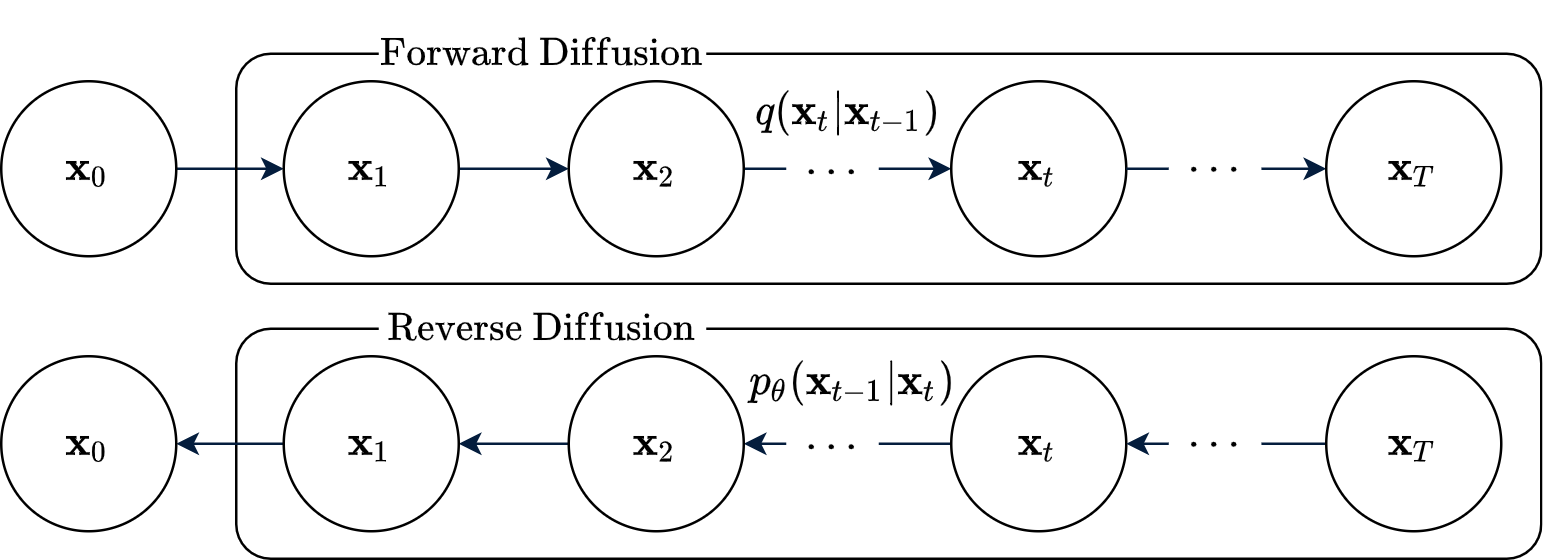
\includegraphics[width=0.65\linewidth]{figs/diffusion_pgm}
	\end{figure}
	\begin{itemize}
		\item Let treat $\bz = (\bx_1, \dots, \bx_T)$ as a latent variable (\textbf{note:} each $\bx_t$ has the same size).
		\item Variational posterior distribution (\textbf{note:} there is no learnable parameters)
		\vspace{-0.4cm}
		\[
			q(\bz | \bx) = q(\bx_1, \dots, \bx_T | \bx_0) = \prod_{t = 1}^T q(\bx_t | \bx_{t - 1}).
		\]
		\vspace{-0.5cm}
		\item Probabilistic model
		\vspace{-0.2cm}
		\[
			p(\bx, \bz | \btheta) = p(\bx | \bz, \btheta) p(\bz | \btheta)
		\]
		\item Generative distribution and prior
		\vspace{-0.3cm}
		\[
			p(\bx | \bz, \btheta) = p(\bx_0 | \bx_1, \btheta); \quad 
			p(\bz | \btheta) = \prod_{t=2}^T p(\bx_{t - 1} | \bx_t, \btheta) \cdot p(\bx_T)
		\]
	\end{itemize}
	\myfootnotewithlink{https://ayandas.me/blog-tut/2021/12/04/diffusion-prob-models.html}{Das A. An introduction to Diffusion Probabilistic Models, blog post, 2021}
\end{frame}
%=======
\begin{frame}{Outline}
	\tableofcontents
\end{frame}
%=======
\section{Denoising diffusion probabilistic model (DDPM)}
%=======
\begin{frame}{Reverse gaussian diffusion process}
	\begin{figure}
		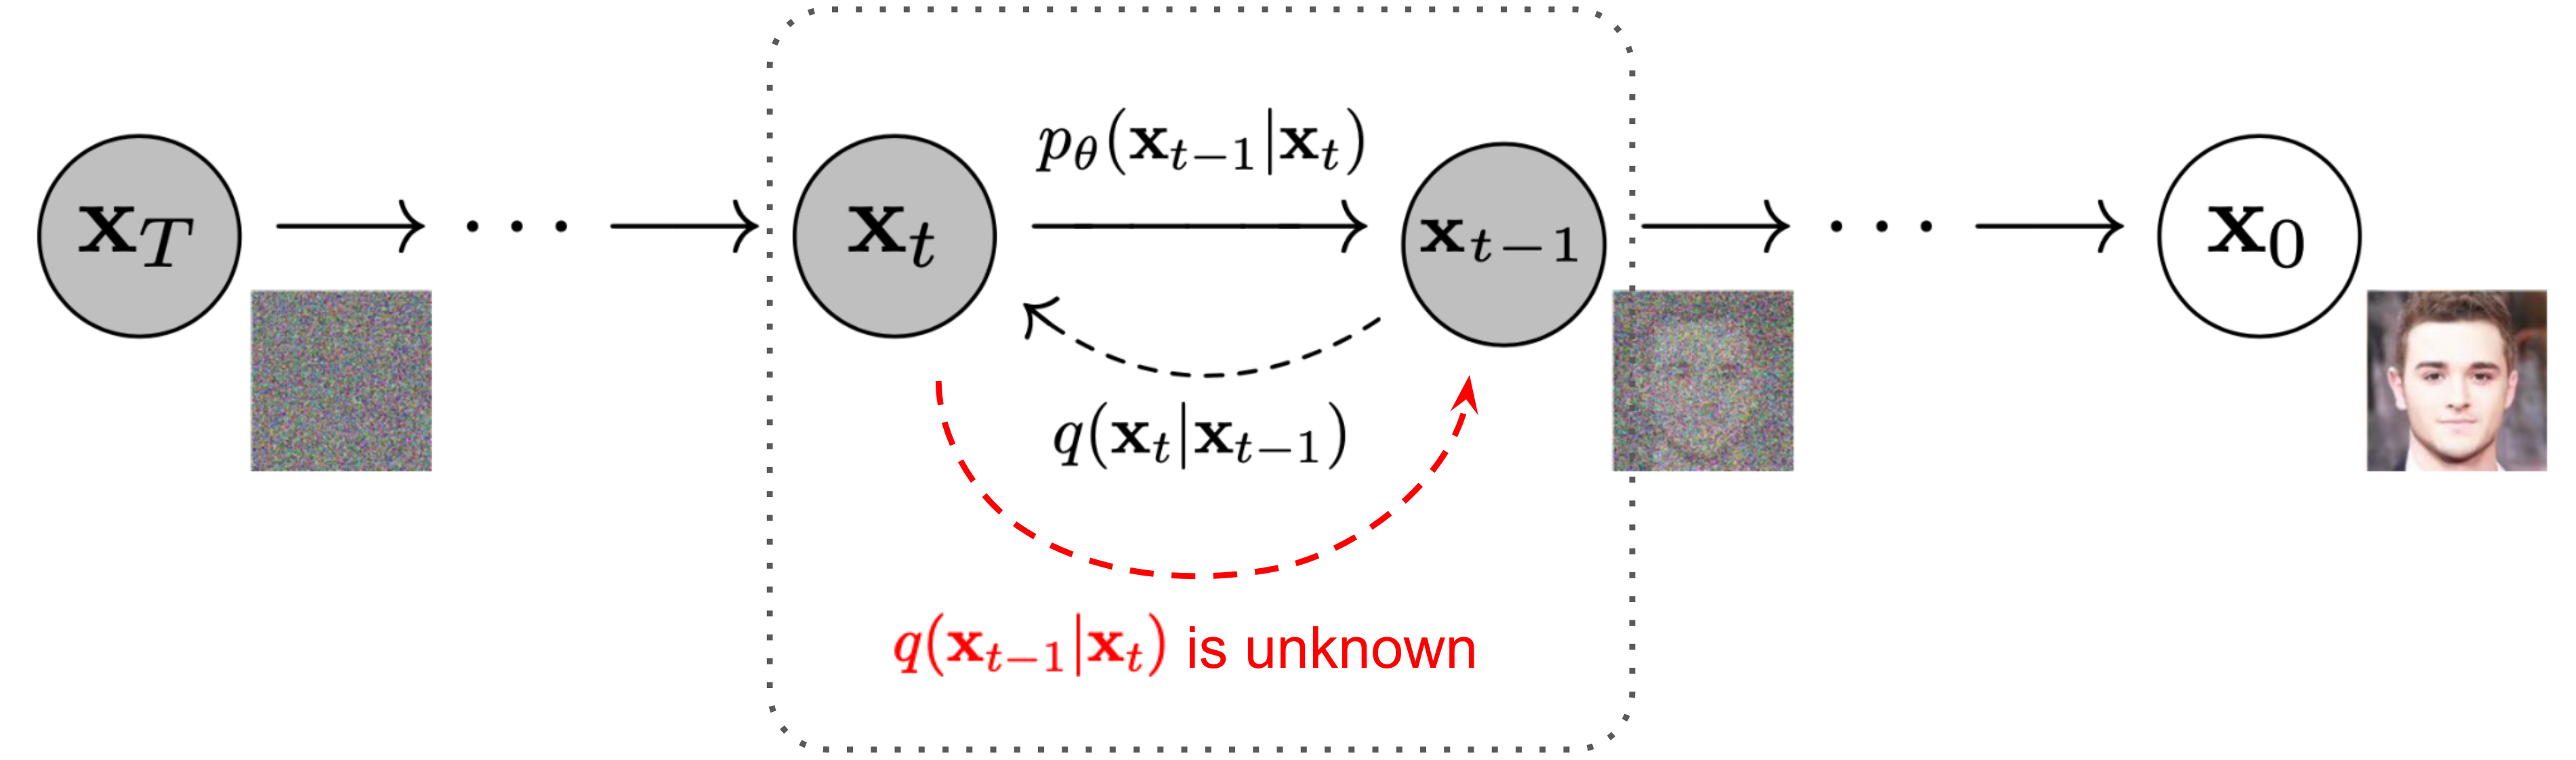
\includegraphics[width=0.8\linewidth]{figs/DDPM}
	\end{figure}
	\vspace{-0.5cm}
	\begin{block}{Forward process}
		\vspace{-0.3cm}
		\[
			q(\bx_t | \bx_{t-1}) = \cN(\bx_t | \sqrt{1 - \beta_t} \cdot \bx_{t-1}, \beta_t \cdot \bI).
		\]
		\vspace{-0.5cm}
	\end{block}
	\begin{block}{Reverse process}
		\vspace{-0.3cm}
		\[
			q(\bx_{t-1}|\bx_{t}) = \frac{q(\bx_{t}|\bx_{t-1}) {\color{violet}q(\bx_{t-1})}}{{\color{violet}q(\bx_{t})}} \approx p(\bx_{t - 1} | \bx_t, \btheta)
		\]
		\vspace{-0.3cm}
		\begin{itemize}
			\item ${\color{violet}q(\bx_{t-1})}$, ${\color{violet}q(\bx_{t})}$ are intractable.
			\item If $\beta_t$ is small enough, $q(\bx_{t-1}|\bx_{t})$ will be Gaussian (Feller, 1949).
		\end{itemize}
	\end{block}
	\myfootnotewithlink{}{Feller W. On the theory of stochastic processes, with particular reference to applications, 1949}
	\end{frame}
%=======
\begin{frame}{Reverse gaussian diffusion process}
	\begin{block}{Reverse process}
		\vspace{-0.6cm}
		\[
			q(\bx_{t-1}|\bx_{t}) \approx p(\bx_{t - 1} | \bx_t, \btheta) = \cN \bigl(\bx_{t - 1} | \bmu(\bx_t, \btheta, t), \bsigma^2(\bx_t, \btheta, t)\bigr)
		\]
		\vspace{-0.6cm}
	\end{block}
	\begin{figure}
		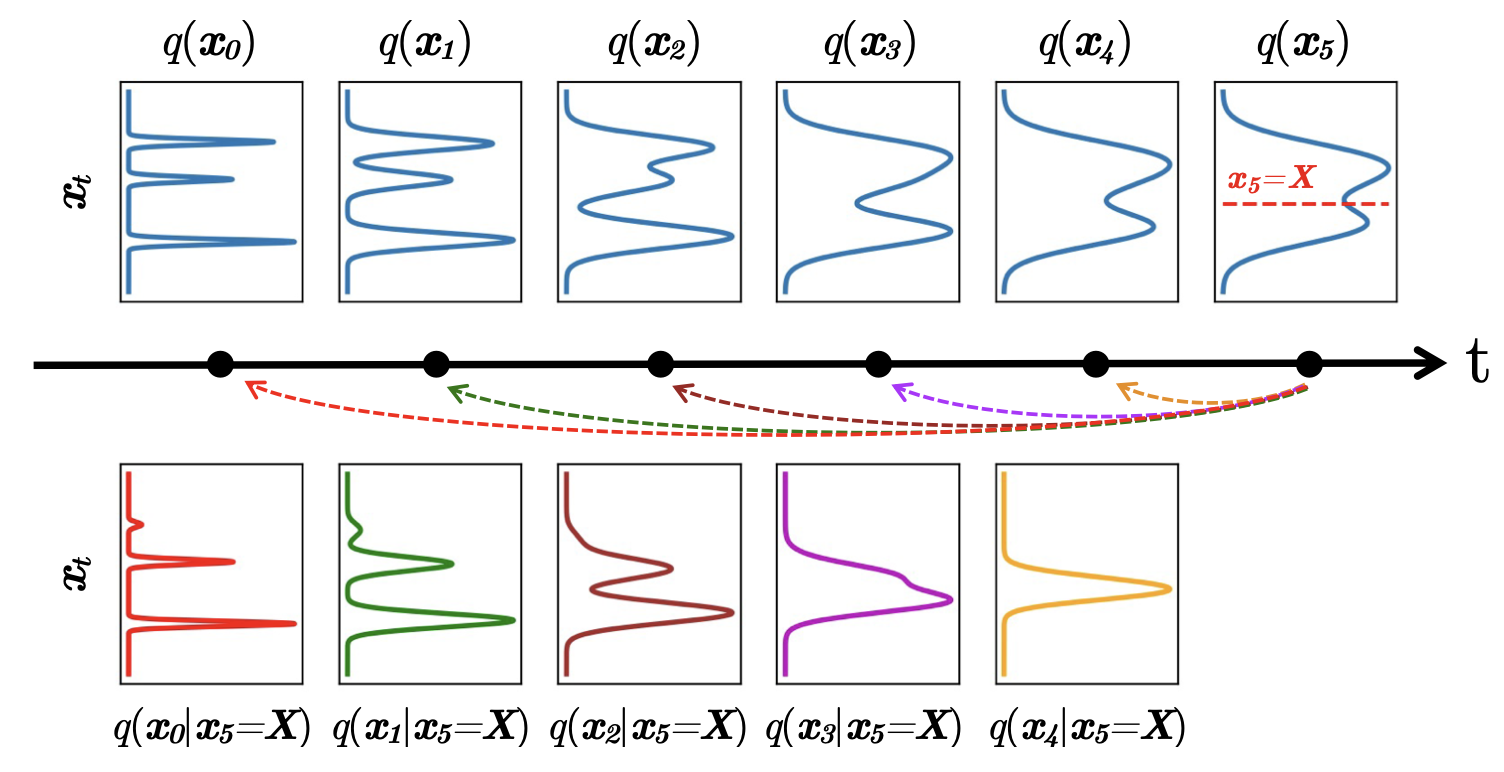
\includegraphics[width=0.7\linewidth]{figs/inverse_distr_1d}
	\end{figure}
	\vspace{-0.3cm}
	\begin{block}{Important distribution}
		\vspace{-0.6cm}
		\[
			q(\bx_{t-1}|\bx_{t}, \bx_0) = \frac{q(\bx_{t}|\bx_{t-1}, {\color{olive}\bx_0}) q(\bx_{t-1} | {\color{olive}\bx_0}) }{q(\bx_{t}| {\color{olive}\bx_0})} = \cN(\tilde{\bmu}_t(\bx_t, \bx_0), \tilde{\beta}_t \bI)
		\]
	\end{block}
	\myfootnotewithlink{https://arxiv.org/abs/2112.07804}{Xiao Z., Kreis K., Vahdat A. Tackling the generative learning trilemma with denoising diffusion GANs, 2021}
	\end{frame}
%=======
\subsection{Objective of DDPM}
%=======
\begin{frame}{Objective of DDPM}
	\begin{block}{ELBO}
		\vspace{-0.4cm}
		\[
			\log p(\bx | \btheta) \geq \bbE_{q({\color{teal}\bz} | \bx)} \log \frac{p(\bx, {\color{teal}\bz} | \btheta)}{q({\color{teal}\bz} | \bx)} = \cL(q, \btheta) \rightarrow \max_{q, \btheta}
		\]
		\vspace{-0.5cm}
	\end{block}
	\begin{block}{Derivation}
		{\small
		\begin{multline*}
			\cL(q, \btheta) = \bbE_{q({\color{teal}\bx_{1:T}} | \bx_0)} \log \frac{p(\bx_0, {\color{teal}\bx_{1:T}} | \btheta)}{q({\color{teal}\bx_{1:T}} | \bx_0)} =  \bbE_{q} \log \frac{{\color{violet}\prod_{t=1}^T} p(\bx_{t-1} | \bx_t, \btheta) {\color{olive}p(\bx_T)} }{{\color{violet}\prod_{t=1}^T} q(\bx_t | \bx_{t-1})}  \\ 
			= \bbE_{q} \left[ \log {\color{olive}p(\bx_T)} + \log \frac{p(\bx_0 | \bx_1, \btheta)}{q(\bx_1 | \bx_0)}  + {\color{violet}\sum_{t=2}^T} \log \left( \frac{p(\bx_{t-1} | \bx_t, \btheta)}{{\color{teal}q(\bx_t | \bx_{t-1})}}\right)\right]
		\end{multline*}
		}
		\vspace{-0.3cm}
		\[
			q(\bx_{t-1}|\bx_{t}, \bx_0) = \frac{{\color{teal} q(\bx_{t}|\bx_{t-1})} q(\bx_{t-1} |\bx_0) }{q(\bx_{t}| \bx_0)} 
		\]
		
		\[
			\log \left( \frac{p(\bx_{t-1} | \bx_t, \btheta)}{{\color{teal}q(\bx_t | \bx_{t-1})}}\right) = \log \left( \frac{p(\bx_{t-1} | \bx_t, \btheta) {\color{teal} q(\bx_{t-1}|\bx_{0})}}{{\color{teal} q(\bx_{t-1}|\bx_{t}, \bx_0) q(\bx_{t}| \bx_0)}}\right)
		\]
	\end{block}
	
	\myfootnotewithlink{https://arxiv.org/abs/2006.11239}{Ho J. Denoising Diffusion Probabilistic Models, 2020}
\end{frame}
%=======
\begin{frame}{Objective of DDPM}
	\begin{block}{Derivation}
		{\small
		\begin{multline*}
			\cL(q, \btheta) = \bbE_{q} \left[ \log p(\bx_T) + \log \frac{p(\bx_0 | \bx_1, \btheta)}{q(\bx_1 | \bx_0)}  + \sum_{t=2}^T \log \left( \frac{p(\bx_{t-1} | \bx_t, \btheta)}{{\color{teal}q(\bx_t | \bx_{t-1})}}\right)\right] \\ 
			= \bbE_{q} \biggl[  \log {\color{violet} p(\bx_T)} + \log \frac{{\color{olive}p(\bx_0 | \bx_1, \btheta)}}{q(\bx_1 | \bx_0)}  + \sum_{t=2}^T \log \left( \frac{p(\bx_{t-1} | \bx_t, \btheta)}{{\color{teal} q(\bx_{t-1}|\bx_{t}, \bx_0)}}\right) + \\ 
			+ \sum_{t=2}^T \log \left( \frac{{\color{teal} q(\bx_{t-1}|\bx_{0})}}{{\color{teal} q(\bx_{t}| \bx_0)}}\right) \biggr] = \bbE_{q} \biggl[ \log \frac{{\color{violet} p(\bx_T)}}{q(\bx_T | \bx_0)} + \log {\color{olive}p(\bx_0 | \bx_1, \btheta)} + \\
			 + \sum_{t=2}^T \log \left( \frac{p(\bx_{t-1} | \bx_t, \btheta)}{q(\bx_{t-1}|\bx_{t}, \bx_0)}\right) \biggr] = \bbE_{q} \biggl[ - KL(q(\bx_T | \bx_0) || p(\bx_T)) + \\
			 + \log p(\bx_0 | \bx_1, \btheta) - \sum_{t=2}^T  KL\bigl( q(\bx_{t-1}|\bx_{t}, \bx_0) || p(\bx_{t-1} | \bx_t, \btheta)\bigr) \biggr]
		\end{multline*}
		}
		\vspace{-0.3cm}
	\end{block}
	\myfootnotewithlink{https://arxiv.org/abs/2006.11239}{Ho J. Denoising Diffusion Probabilistic Models, 2020}
\end{frame}
%=======
\begin{frame}{Objective of DDPM}
		\vspace{-0.6cm}
		\begin{multline*}
			\cL(q, \btheta) =  \bbE_{q} \Bigl[ {\color{olive}\log p(\bx_0 | \bx_1, \btheta)} - {\color{violet}KL\bigl(q(\bx_T | \bx_0) || p(\bx_T)\bigr)} - \\
			- \sum_{t=2}^T \underbrace{KL \bigl(q(\bx_{t-1} | \bx_t, \bx_0) || p(\bx_{t - 1} | \bx_t, \btheta )\bigr)}_{\cL_t} \Bigr]
		\end{multline*}
		\vspace{-0.5cm}
	\begin{itemize}
		\item {\color{olive}First term} is a decoder distribution
		\[
			\log p(\bx_0 | \bx_1, \btheta) = \log \cN \bigl(\bx_0 | \bmu(\bx_1, \btheta, t), \bsigma^2(\bx_1, \btheta, t)\bigr)
		\] 
		\item {\color{violet}Second term} is constant ($p(\bx_T)$ is a standard Normal, $q(\bx_T | \bx_0)$ is a non-parametrical Normal).
		\item $\cL_t$ is a KL between two normal distributions:
		\[
			q(\bx_{t-1} | \bx_t, \bx_0) = \cN(\bx_{t-1} | \tilde{\bmu}_t(\bx_t, \bx_0), \tilde{\beta}_t \bI),
		\]
		$\tilde{\bmu}_t(\bx_t, \bx_0)$ and $\tilde{\beta}_t$ have analytical formulas (we omit it) and they are both dependent on $\beta_t$.
	\end{itemize}
	\myfootnotewithlink{https://arxiv.org/abs/2006.11239}{Ho J. Denoising Diffusion Probabilistic Models, 2020}
\end{frame}
%=======
\subsection{Reparametrization of DDPM}
%=======
\begin{frame}{Gaussian diffusion model as VAE}
	\vspace{-0.5cm}
	\begin{align*}
		q(\bx_{t-1} | \bx_t, \bx_0) &= \cN(\bx_{t-1} | \tilde{\bmu}_t(\bx_t, \bx_0), \tilde{\beta}_t \bI), \\
		p(\bx_{t - 1} | \bx_t, \btheta) &= \cN \bigl(\bx_{t - 1} | \bmu(\bx_t, \btheta, t), \bsigma^2(\bx_t, \btheta, t)\bigr)
	\end{align*}
	\vspace{-0.5cm}
	\begin{itemize}
		\item Assume $\bsigma^2(\bx_t, \btheta, t) = \tilde{\beta}_t \bI$.
		\item Use KL formula between two normal distributions:
		\begin{align*}
			\cL_t &= KL\Bigl(\cN\bigl(\tilde{\bmu}_t(\bx_t, \bx_0), \tilde{\beta}_t \bI \bigr) || \cN\bigl(\bmu(\bx_t, \btheta, t), \tilde{\beta}_t \bI\bigr)\Bigr) \\ 
			&= \bbE_{\bepsilon} \left[ \frac{1}{2\tilde{\beta}_t} \bigl\| \tilde{\bmu}_t(\bx_t, \bx_0) - \bmu(\bx_t, \btheta, t) \bigr\|^2 \right] \\
			& = \bbE_{\bepsilon} \left[ \frac{1}{2\tilde{\beta}_t} \left\| {\color{violet} \frac{1}{\sqrt{1 - \beta_t}}\left( \bx_t - \frac{\beta_t}{\sqrt{1 - \bar{\alpha}_t} } \bepsilon \right)} - \bmu(\bx_t, \btheta, t) \right\|^2 \right]
		\end{align*}
		 {\color{gray}Here we used the analytic expression for $\tilde{\bmu}_t(\bx_t, \bx_0)$.}
	\end{itemize}
	\begin{block}{Reparametrization}
		\vspace{-0.3cm}
		\[
			\bmu(\bx_t, \btheta, t) = \frac{1}{\sqrt{1 - \beta_t}}\left( \bx_t - \frac{\beta_t}{\sqrt{1 - \bar{\alpha}_t} } \bepsilon(\bx_t, \btheta, t) \right) 
		\]
		\vspace{-0.6cm}
	\end{block}
	\myfootnotewithlink{https://arxiv.org/abs/2006.11239}{Ho J. Denoising Diffusion Probabilistic Models, 2020}
	\end{frame}
%=======
\begin{frame}{Reparametrization of DDPM}
	\begin{block}{KL term}
		\vspace{-0.8cm}
		\begin{multline*}
			\cL_t = \bbE_{\bepsilon} \biggl[ \frac{1}{2\tilde{\beta}_t} \Bigl\| {\color{violet} \frac{1}{\sqrt{1 - \beta_t}}\left( \bx_t - \frac{\beta_t}{\sqrt{1 - \bar{\alpha}_t} } \bepsilon \right)} - \\
			- \frac{1}{\sqrt{1 - \beta_t}}\left( \bx_t - \frac{\beta_t}{\sqrt{1 - \bar{\alpha}_t} } \bepsilon(\bx_t, \btheta, t) \right)  \Bigr\|^2 \biggr] = \\
			\bbE_{\bepsilon} \left[ \frac{\beta_t^2}{2\tilde{\beta}_t (1 - \beta_t)} \left\| \frac{\bepsilon}{\sqrt{1 - \bar{\alpha}_t}} - \frac{\bepsilon({\color{teal}\bx_t}, \btheta, t)}{\sqrt{1 - \bar{\alpha}_t}}\right\|^2 \right]
		\end{multline*}
	\end{block}
		\vspace{-0.5cm}
		\[
			{\color{teal}\bx_t} = \sqrt{\bar{\alpha}_t} \cdot \bx_{0} + \sqrt{1 - \bar{\alpha}_t} \cdot \bepsilon, \quad \text{where } \bepsilon \sim \cN(0, 1)
		\]
	At each step of reverse diffusion process we try to predict the noise $\bepsilon$ that we used in forward process!
	\myfootnotewithlink{https://arxiv.org/abs/2006.11239}{Ho J. Denoising Diffusion Probabilistic Models, 2020}
\end{frame}
%=======
\begin{frame}{Gaussian diffusion model vs Score matching}
	\vspace{-0.3cm}
	\[
		\cL_t = {\color{olive}\bbE_{\bepsilon}} \left[ \frac{\beta_t^2}{2\tilde{\beta}_t (1 - \beta_t)} \left\| {\color{violet}\frac{\bepsilon}{\sqrt{1 - \bar{\alpha}_t}}} - {\color{teal}\frac{\bepsilon(\bx_t, \btheta, t)}{\sqrt{1 - \bar{\alpha}_t}}}\right\|^2 \right]
	\]
	\begin{itemize}
		\item Result from Statement 2
		\[
			q(\bx_t | \bx_0) = \cN(\bx_t | \sqrt{\bar{\alpha}_t} \cdot \bx_0, (1 - \bar{\alpha}_t) \cdot \bI).
		\]
		\item Score of noised distribution
		\[
			\nabla_{\bx_t} \log q(\bx_t | \bx_0) = - \frac{\bepsilon}{\sqrt{1 - \bar{\alpha}_t}}, \quad \text{where } \bepsilon \sim \cN(0, 1).
		\]
		\item Let reparametrize our model: 
		\[
			\bs(\bx_t, \btheta, t) = - \frac{\bepsilon(\bx_t, \btheta, t)}{\sqrt{1 - \bar{\alpha}_t}}.
		\]
	\end{itemize}
	\begin{block}{Noise conditioned score network}
		\vspace{-0.2cm}
		\[
			{\color{olive}\bbE_{p(\bx' | \bx, \sigma_l)}}\bigl\| {\color{teal}\bs(\bx', \btheta, \sigma_l)} - {\color{violet}\nabla_{\bx'} \log p(\bx' | \bx, \sigma_l)} \bigr\|^2_2 \rightarrow \min_{\btheta}
		\]
	\end{block}
	\myfootnotewithlink{https://arxiv.org/abs/2006.11239}{Ho J. Denoising Diffusion Probabilistic Models, 2020}
	\end{frame}
%=======
\subsection{Overview}
%=======
\begin{frame}{Denoising diffusion probabilistic model (DDPM)}
	\begin{block}{DDPM is a VAE model}
		\begin{itemize}
			\item Encoder is a fixed Gaussian Markov chain.
			\item Latent variable is a hierarchical (in each step the dim. of the latent equals to the dim of the input).
			\item Decoder is a simple Gaussian model.
			\item Prior distribution is given by parametric Gaussian Makov chain.
		\end{itemize}
	\end{block}
	\begin{minipage}{0.5\linewidth}
		\begin{block}{Forward process}
			\begin{enumerate}
				\item $\bx_0 = \bx \sim \pi(\bx)$;
				\item $\bx_t = \sqrt{1 - \beta} \cdot \bx_{t - 1} + \sqrt{\beta} \cdot \bepsilon$, where $\bepsilon \sim \cN(0, 1)$, $t \geq 1$;
				\item $\bx_T \sim p_{\infty}(\bx) = \cN(0, 1)$.
			\end{enumerate}
		\end{block}
	\end{minipage}%
	\begin{minipage}{0.5\linewidth}
		\begin{block}{Reverse process}
			\begin{enumerate}
				\item $\bx_T \sim p_{\infty}(\bx) = \cN(0, 1)$;
				\item $\bx_{t - 1} = \bsigma(\bx_t, \btheta, t) \cdot \bepsilon + \bmu(\bx_t, \btheta, t)$;
				\item $\bx_0 = \bx \sim \pi(\bx)$;
			\end{enumerate}
		\end{block}
	\end{minipage}
\end{frame}
%=======
\begin{frame}{Denoising diffusion probabilistic model (DDPM)}
	\begin{block}{Samples}
		\begin{figure}
			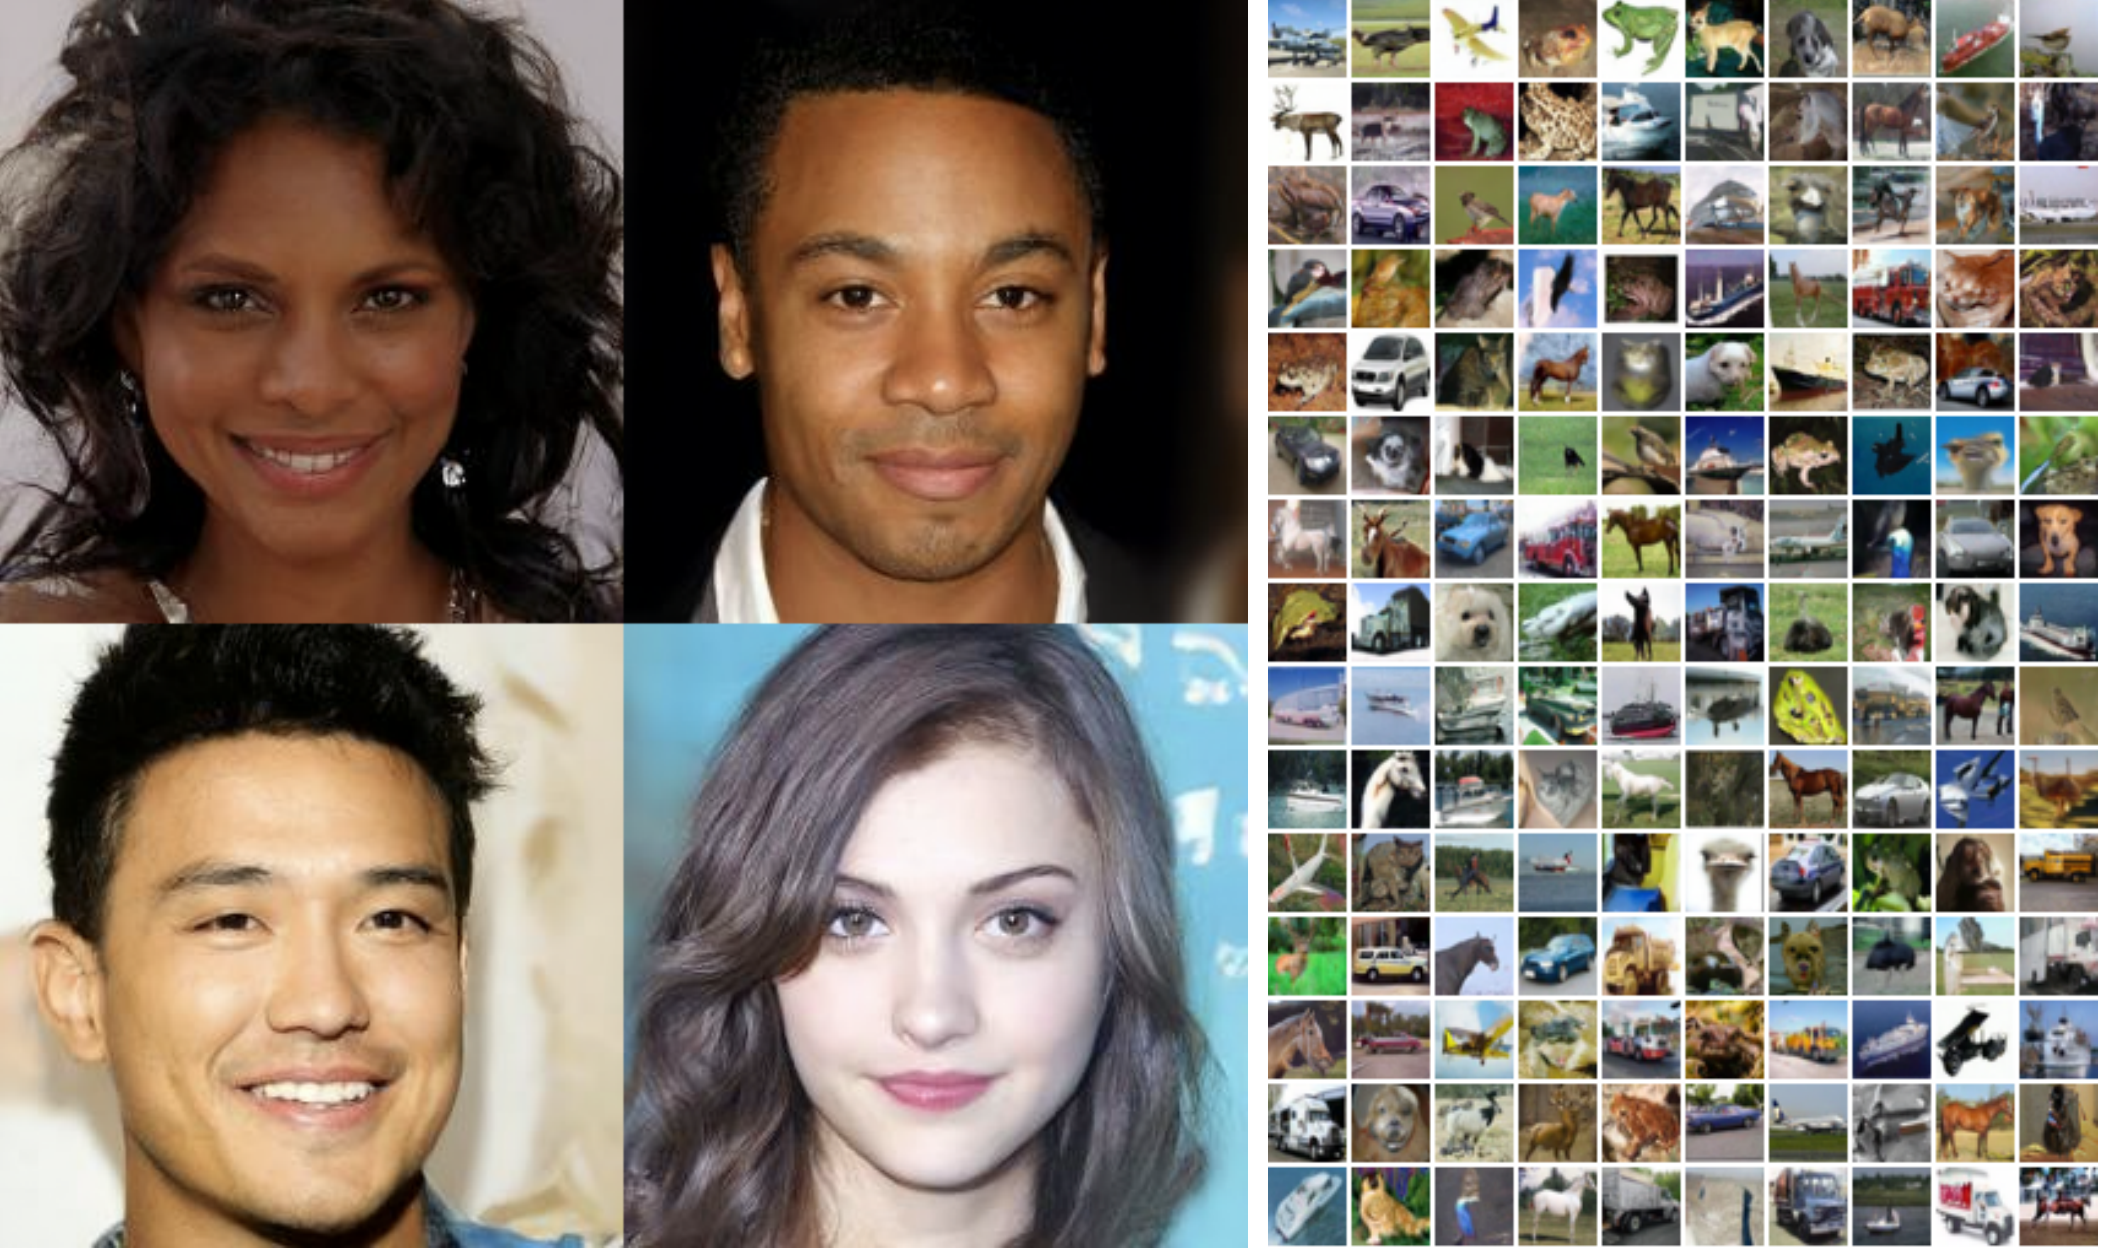
\includegraphics[width=\linewidth]{figs/ddpm_samples}
		\end{figure}
	\end{block}
	\myfootnotewithlink{https://arxiv.org/abs/2006.11239}{Ho J. Denoising Diffusion Probabilistic Models, 2020}
\end{frame}
%=======
\section{The worst course overview}
%=======
\begin{frame}{The worst course overview :)}
	\begin{figure}
		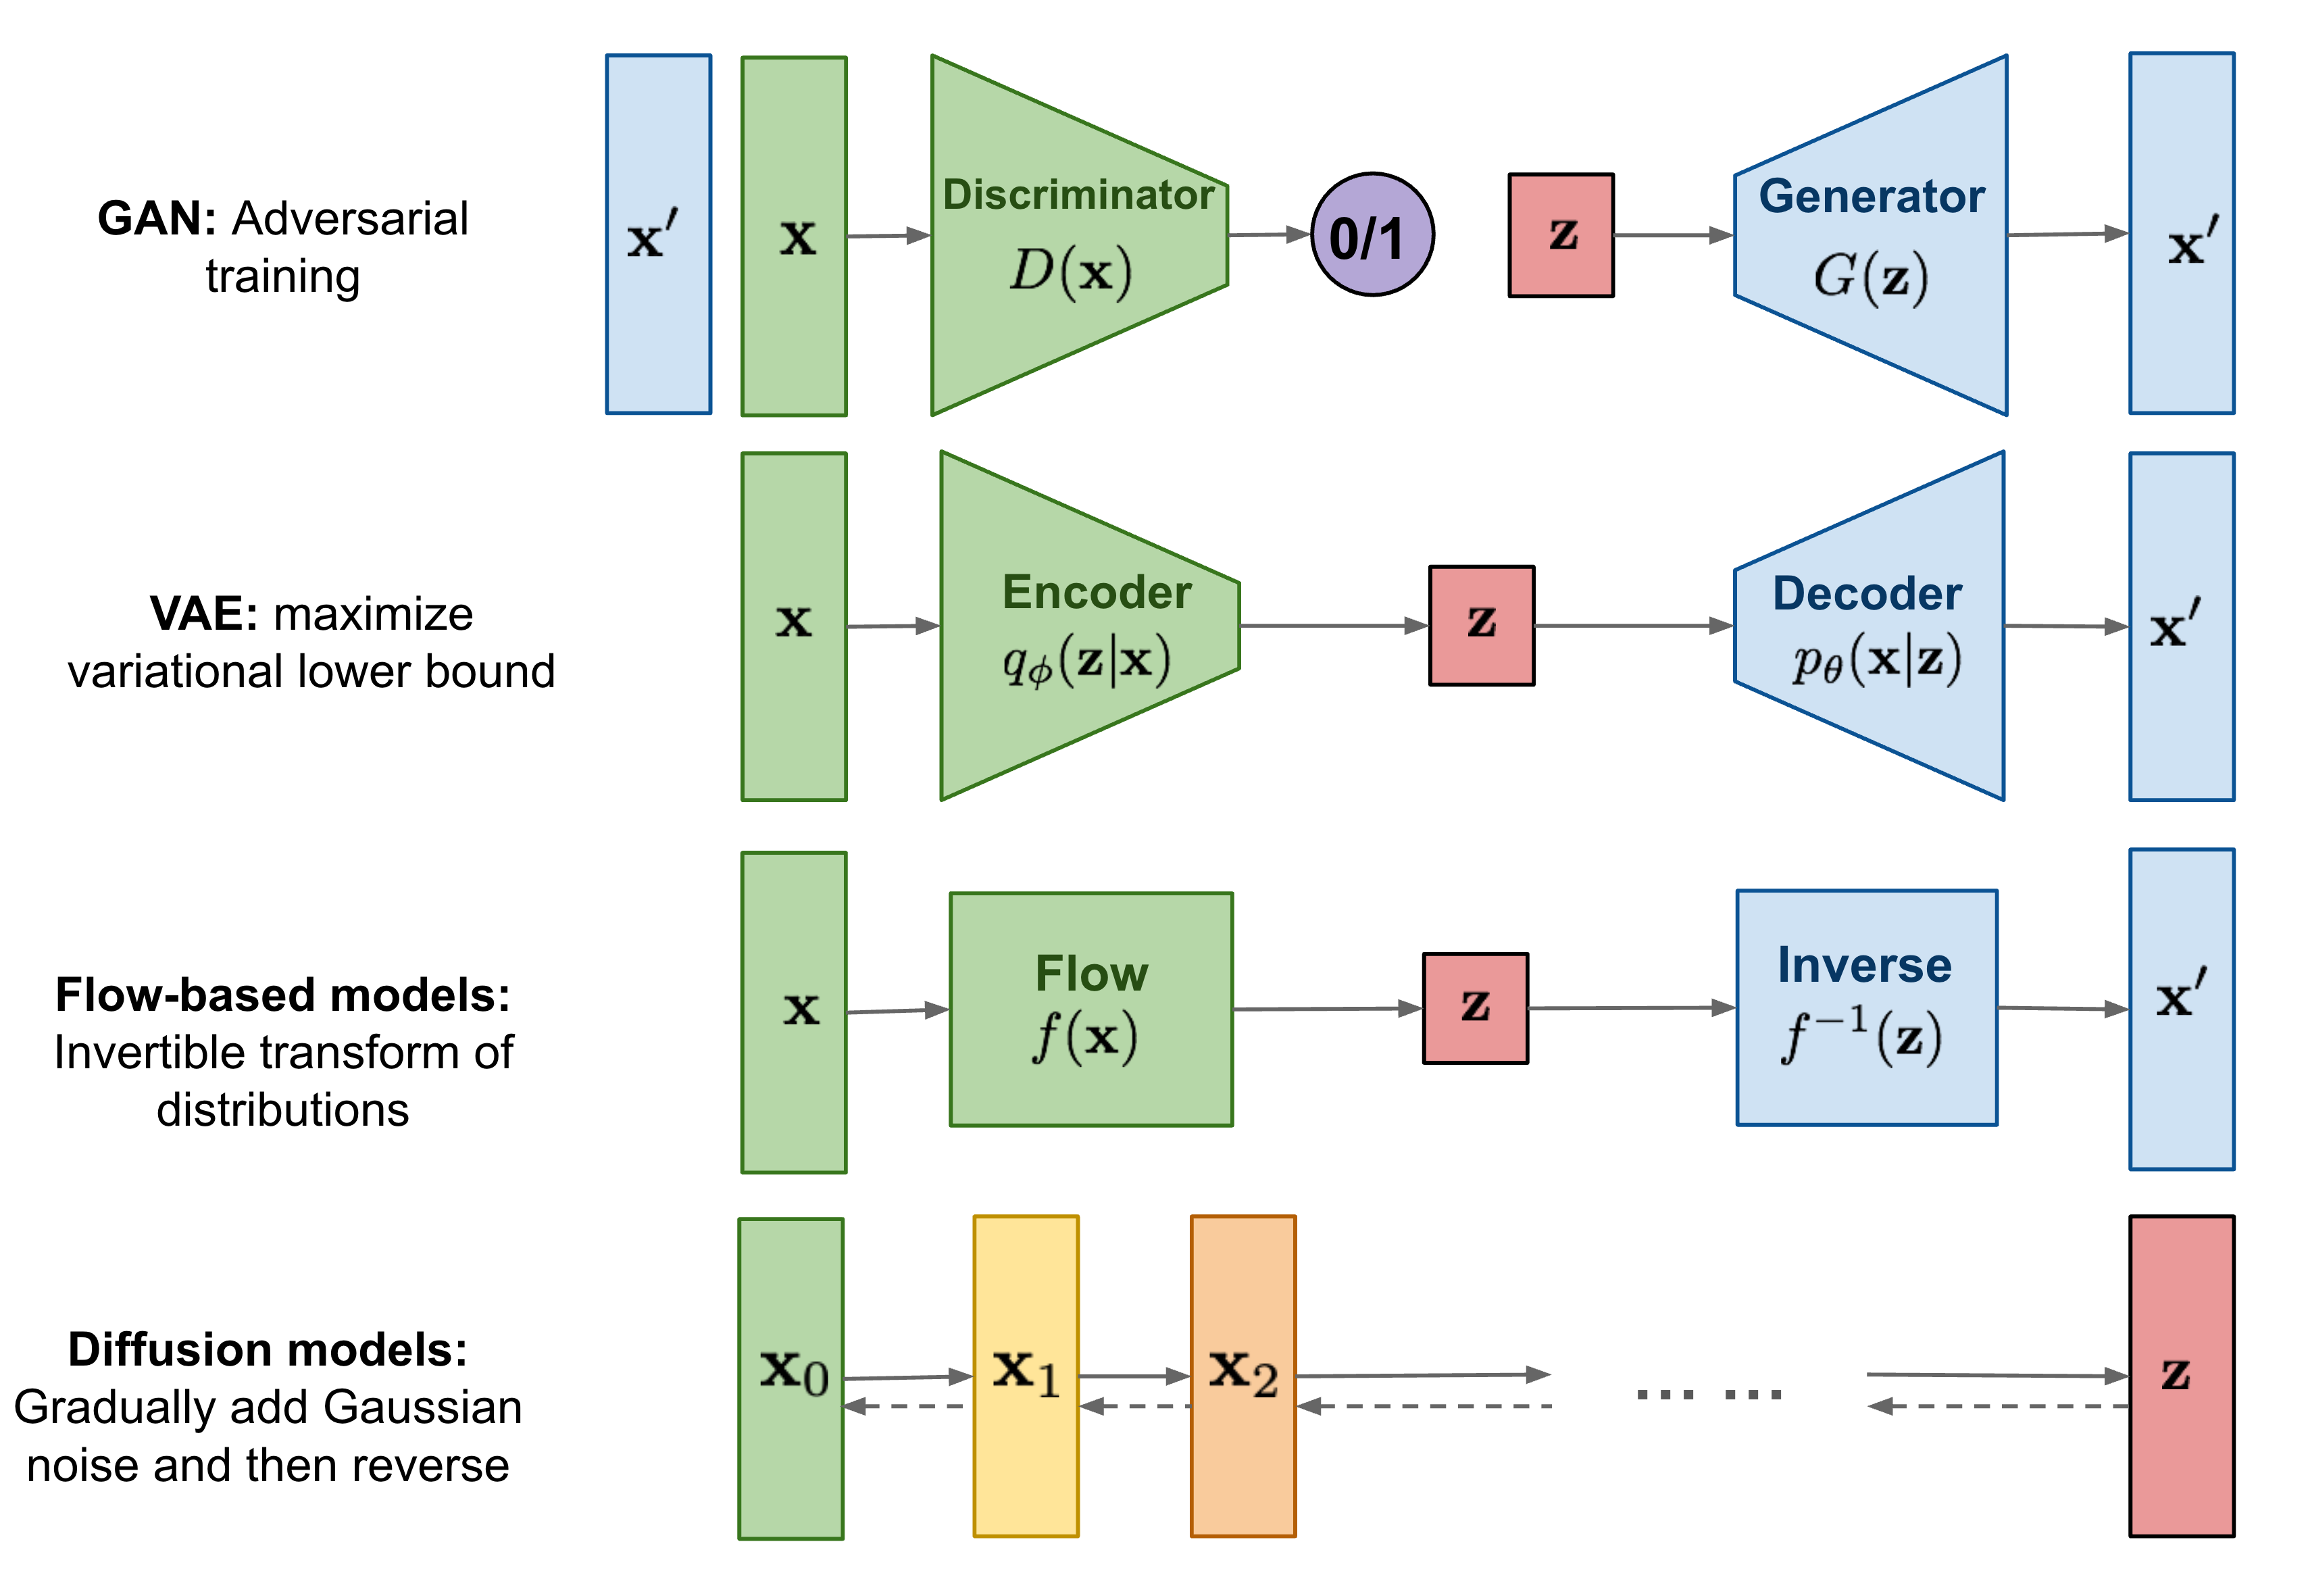
\includegraphics[width=\linewidth]{figs/generative-overview}
	\end{figure}
	\myfootnotewithlink{https://lilianweng.github.io/posts/2021-07-11-diffusion-models/}{Weng L. What are Diffusion Models?, blog post, 2021}
\end{frame}
%=======
\begin{frame}{The worst course overview :)}
	\begin{figure}
		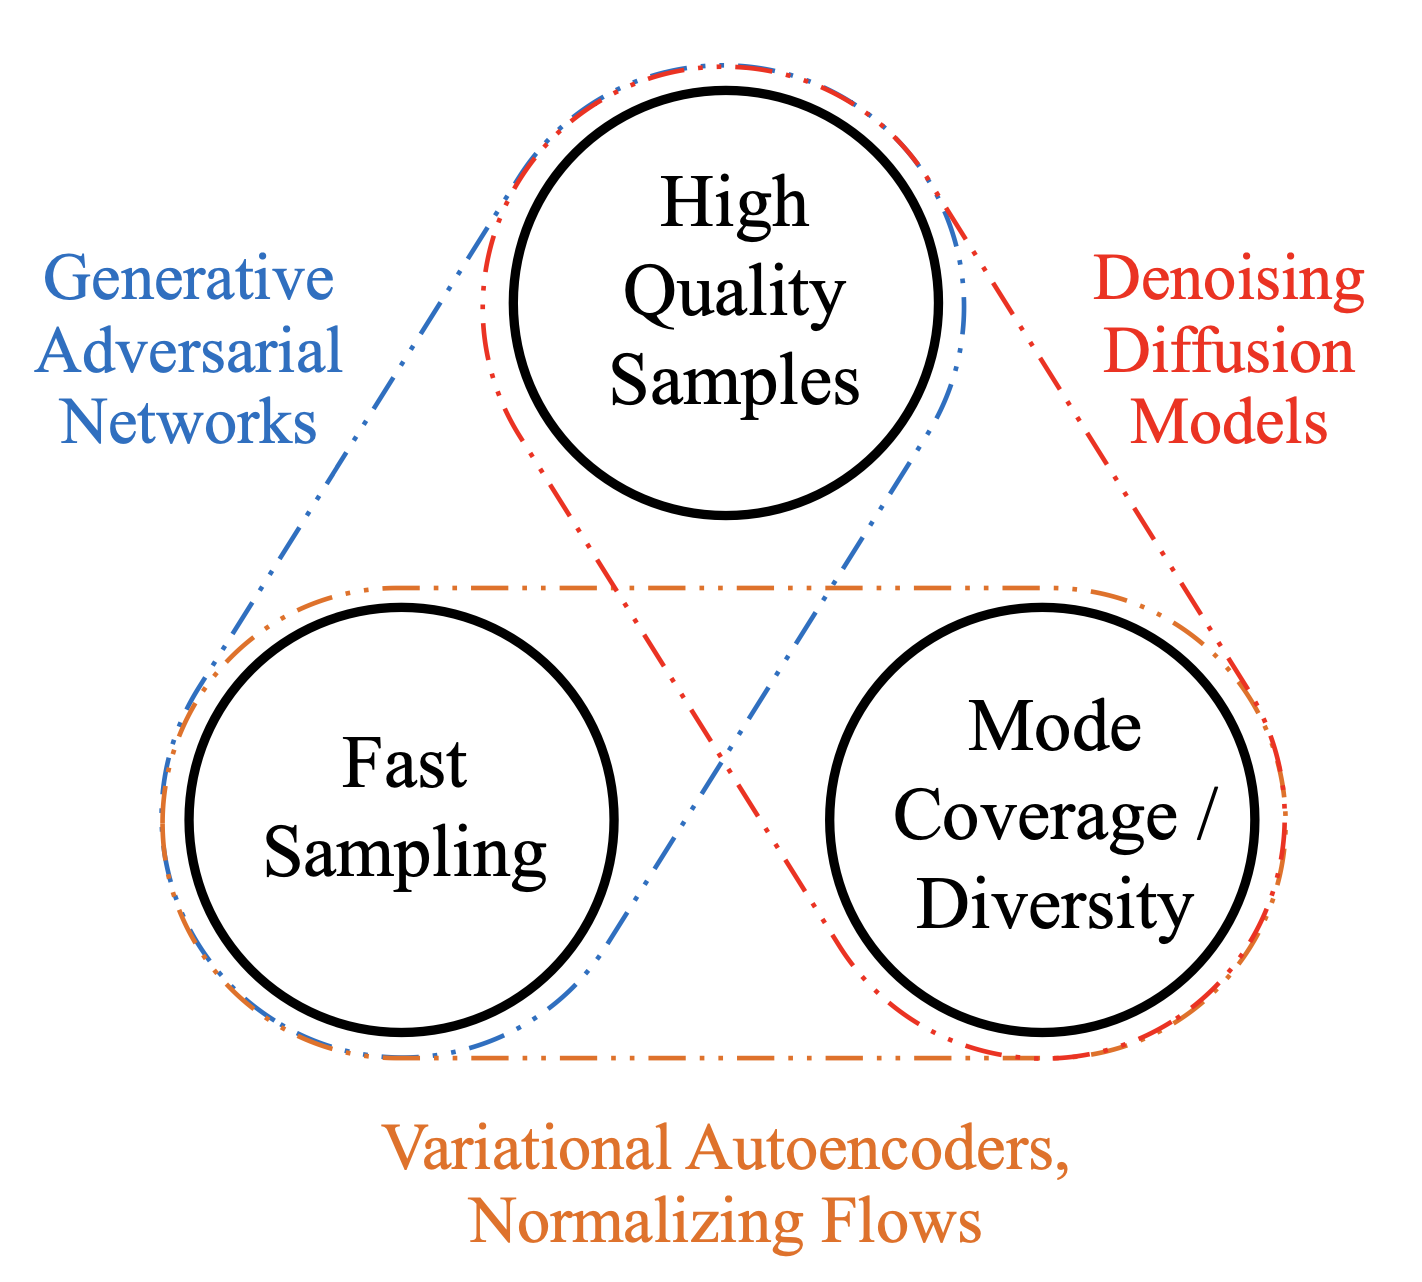
\includegraphics[width=0.7\linewidth]{figs/trilemma}
	\end{figure}
	\myfootnotewithlink{https://arxiv.org/abs/2112.07804}{Xiao Z., Kreis K., Vahdat A. Tackling the generative learning trilemma with denoising diffusion GANs, 2021}
\end{frame}
%=======
\begin{frame}{Summary}
	\begin{itemize}
		\item Diffusion model is a VAE model which reverts gaussian diffusion process using variational inference.
		\vfill
		\item ELBO of DDPM is a sum of KL terms.
		\vfill
		\item At each step DDPM predicts the noise used in forward process.
		\vfill
		\item Objective of DDPM is closely related to the noise conditioned score network and score matching.
	\end{itemize}
\end{frame}
\end{document} 